\documentclass{beamer}
\usefonttheme{professionalfonts}
\usefonttheme{serif}
\usepackage{mathtools}
\usepackage{tikz}
\usepackage{pgfplots}
\usetikzlibrary{arrows,backgrounds,shapes,matrix,positioning,fit}
\usetikzlibrary{decorations.markings}
\usepackage{caption}
\usepackage{subcaption}
% For maths
\usepackage{amsmath}
\usepackage{amssymb}
% For Figures
\usepackage{graphicx}
% For including source codes
\usepackage{listings}
\usepackage{color}
\setbeamertemplate{bibliography item}{[\theenumiv]}

\mode<presentation>
{
  \usetheme{CambridgeUS}
  %\useoutertheme{infolines} % Showing only current section in navigation
  \setbeamertemplate{headline}{}  % Empty headline
  \setbeamertemplate{footline}[frame number]  % Getting rid of footer items except slide number
  \setbeamercovered{invisible}
  \beamertemplatenavigationsymbolsempty % Getting rid of navigation bullets at the bottom
}

\title[IQ Modulator]{IQ Modulator Board}
\author[Manu]
{
  Manu T S\\
  \href{mailto:manu.ts@ee.iitb.ac.in}{manu.ts@ee.iitb.ac.in}
}
\institute[IIT Bombay]
{
  Department of Electrical Engineering\\
  Indian Institute of Technology Bombay
}
\date{\today}

\begin{document}

\begin{frame}
  \titlepage
\end{frame}

\begin{frame}{IQ Modulation}
  Any passband signal $s_{\text{p}}(t)$ can be written as
  \pause
  \begin{equation}
      s_{\text{p}}(t) = \sqrt{2}s_{\text{i}}(t)\operatorname{cos}(2\pi f_ct) - \sqrt{2}s_{\text{q}}(t)\operatorname{sin}(2\pi f_ct) \nonumber
  \end{equation}
  \pause
  where,
  \begin{equation}
    s(t) = s_{\text{i}}(t) + \text{j}s_{\text{q}}(t) \nonumber
  \end{equation}
  \pause
  is called the complex envelope of $s_{\text{p}}(t)$.
\end{frame}

\begin{frame}{IQ Modulation}
\begin{figure}
    \centering
      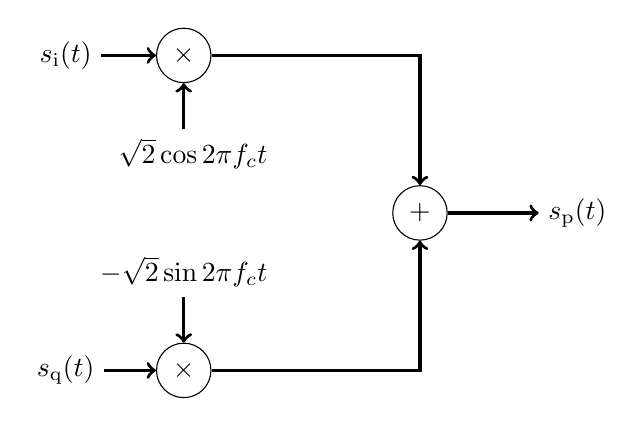
\begin{tikzpicture}[scale=1.0,transform shape]
      \node at (-0.5,2) (sc) {$s_{\text{i}}(t)$};
      \node at (-0.5,-2) (ss) {$s_{\text{q}}(t)$};
      \node[circle, draw, minimum size = 5mm] at (1,2) (prodc) {$\times$};
      \node[circle, draw, minimum size = 5mm] at (1,-2) (prods) {$\times$};
      \node[circle, draw, minimum size = 5mm] at (4,0) (adder) {$+$};
      \node at (1,0.75) (cos) {$\ \ \sqrt{2}\cos 2\pi f_ct$};
      \node at (1,-0.75) (sin) {$-\sqrt{2}\sin 2\pi f_ct$};
      \node at (6,0) (sp) {$s_{\text{p}}(t)$};
      \draw[->,very thick] (sc) -- (prodc);
      \draw[->,very thick] (ss) -- (prods);
      \draw[->,very thick] (prodc) -| (adder);
      \draw[->,very thick] (prods) -| (adder);
      \draw[->,very thick] (cos) -- (prodc);
      \draw[->,very thick] (sin) -- (prods);
      \draw[->,very thick] (adder) -- (sp);
      \end{tikzpicture}
%    \caption{Up-conversion: Getting passband signal from complex envelope
%    \label{fig:upconversion}}
  \end{figure}
\end{frame}

\end{document}
